\documentclass{article}

%\usepackage[english]{babel}%

\usepackage{graphicx}

\usepackage{tabulary}

\usepackage{tabularx}

\usepackage[table,xcdraw]{xcolor}

\usepackage{pdflscape}

\usepackage{float}

\usepackage{lastpage}

\usepackage{multirow}

\usepackage{xcolor}

\usepackage{cancel}

\usepackage{amsmath}

\usepackage[table]{xcolor}

\usepackage{fixltx2e}

\usepackage[T1]{fontenc}

\usepackage[utf8]{inputenc}

\usepackage{ifthen}

\usepackage{fancyhdr}

\usepackage[document]{ragged2e}

\usepackage[margin=1in,top=1.2in,headheight=57pt,headsep=0.1in]
{geometry}

\usepackage{ifthen}

\usepackage{fancyhdr}

\everymath{\displaystyle}

\usepackage[document]{ragged2e}

\usepackage{fancyhdr}

\usepackage{mathabx}

\usepackage[shortlabels]{enumitem}
\usepackage{tikz}
\usepackage{mwe}
\usetikzlibrary{calc}
\usetikzlibrary{shapes.multipart, shapes.geometric, arrows}
\usetikzlibrary{calc, decorations.markings}
\usetikzlibrary{arrows.meta}
\usetikzlibrary{shapes,snakes}
\usetikzlibrary{quotes,angles, positioning}

\everymath{\displaystyle}

\linespread{2}%controls the spacing between lines. Bigger fractions means crowded lines%

%\pagestyle{fancy}

%\usepackage[margin=1 in, top=1in, includefoot]{geometry}

%\everymath{\displaystyle}

\linespread{1.3}%controls the spacing between lines. Bigger fractions means crowded lines%

%\pagestyle{fancy}

\pagestyle{fancy}

\setlength{\headheight}{56.2pt}

\usepackage{soul}

 

\chead{\ifthenelse{\value{page}=1}{
\includegraphics[scale=0.3]{BassettCTCLogo}\\ \textbf \textbf Pop Quiz Week 4}}

\rhead{\ifthenelse{\value{page}=1}{Name: \rule{4cm}{0.05cm}}{}}

\lhead{\ifthenelse{\value{page}=1}{Water Distribution - January 2023}{Pop Quiz Week 4}}

\rfoot{\ifthenelse{\value{page}=1}{}{}}

 

\cfoot{}

\lfoot{Page \thepage\ of \pageref{LastPage}}

\renewcommand{\headrulewidth}{2pt}

\renewcommand{\footrulewidth}{1pt}

\begin{document}

 


\begin{enumerate}

\item A 12 gpm alum solution is being added to coagulate a 1,500 gpm influent water flow stream resulting in an alum dose of 25 mg/l.  What is \% concentration of the alum solution?

\vspace{0.3cm}
\begin{tikzpicture}

\draw [-] (-3.2,4.2) -- (-0.4,4.2);
\draw [->] (-0.2,4) -- (-0.2,1.9);
\draw [->] (-3.2,1.9) -- (4,1.9);
\draw [shift={(-0.4,4)}] plot[domain=0:1.57,variable=\t]({1*0.2*cos(\t r)+0*0.2*sin(\t r)},{0*0.2*cos(\t r)+1*0.2*sin(\t r)});
\draw (-3.1,4.1) node[anchor=north west] {V$_{\tiny{Alum}}$=$12 gpm$};
\draw (-3.1,3.6) node[anchor=north west] {C$_{\tiny{Alum}}$ = ?};
\draw (-4.2,4.5) node[anchor=north west] {Alum};
\draw (-4.2,2.2) node[anchor=north west] {Water};
\draw (-2.1,1.8) node[anchor=north west] {$1500 gpm$};
\draw (0.7,1.8) node[anchor=north west] {C$_2$=25ppm Alum};
\draw (0.7,1.3) node[anchor=north west] {V$_2$=12+1500=1,512 gpm};
\end{tikzpicture}\\
\vspace{0.2cm}
C$_1$ * V$_1$ = C$_2$ * V$_2$ \\
\vspace{0.2cm}
C$_{\tiny{Alum}}$ * V$_{\tiny{Alum}}$  =  C$_2$ * (V$_{\tiny{Alum}}$+V$_{\tiny{Water}}$)\\
\vspace{0.2cm}
C$_{\tiny{Alum}}$ * 12 =  25 * (1,512)\\
\vspace{0.2cm}
C$_{\tiny{Alum}}=\dfrac{25 * (804.3)}{4.3}=\boxed{3,150 \enspace \mathrm{ppm} \enspace \mathrm{or} \enspace 0.32\%}$\\
\vspace{0.3cm}
\newpage
\item The 600 gpm source water stream with an arsenic concentration of 9 mg/l is to be blended with another source water stream flowing at 300 gpm containing 4 mg/l arsenic.  Calculate the arsenic concentration in the blended stream.

Solution:\\
\vspace{0.2cm}
C$_1$ * V$_1$ + C$_2$ * V$_2$ + =  C$_3$ * V$_3$=C$_3$*(V$_1$ + V$_2$)\\
\vspace{0.2cm}
C$_{Source \enspace 1}$ * V$_{Source \enspace 1}$ + C$_{Source \enspace 2}$ * V$_{Source \enspace 2}$ =  C$_{Blend}$ * V$_{Blend}$=C$_{Blend}$*(V$_{Source \enspace1}$ + V$_{Source \enspace 2}$)\\
\vspace{0.3cm}
$\implies C_{Blend}=\dfrac{C_{Source \enspace 1} * V_{Source \enspace 1} + C_{Source \enspace 2} * V_{Source \enspace 2}}{V_{Source \enspace 1} + V_{Source \enspace 2}}=\dfrac{9*600+4*300}{600+300}=\boxed{7.3 \enspace \textrm{mg/l}}$

\newpage
\item    For a pumping system given the following information: \\
Total Static Head $=50$ feet\\
Friction Loss $=5$ feet\\
Pump Rate $=300$ gpm\\
Pump Efficiency $=92 \%$\\
Motor Efficiency $=85 \%$\\
Calculate: \\
1) Brake Hp, and \\
2) Input Hp\\
\vspace{0.3cm}
Solution:\\
 \vspace{0.4cm}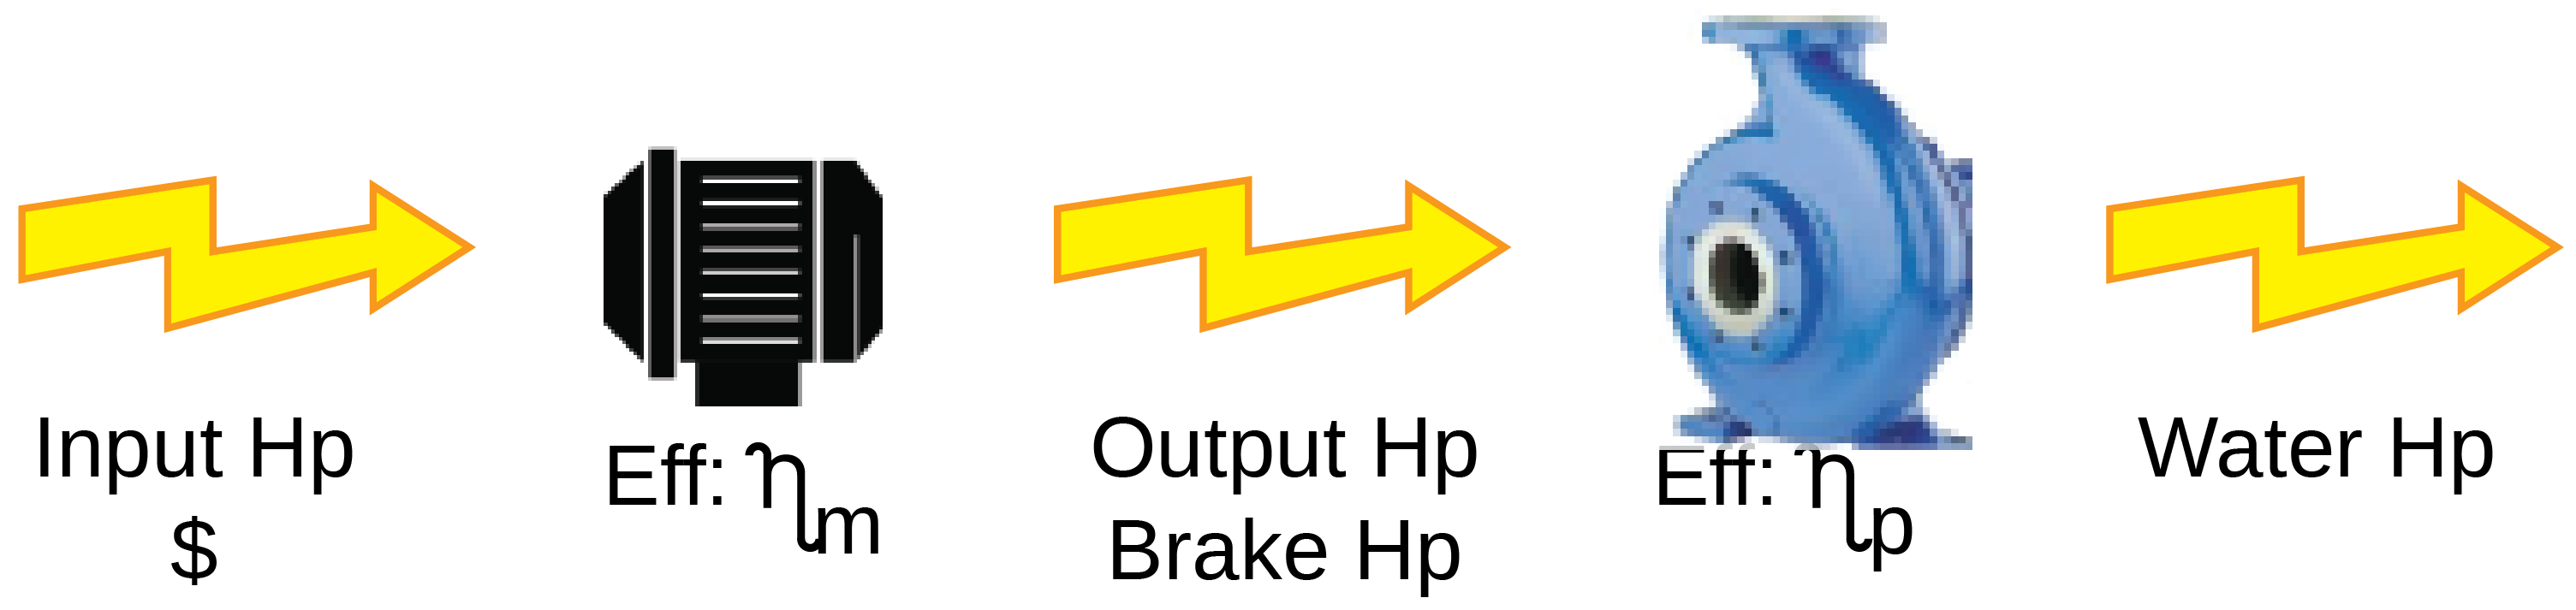
\includegraphics[scale=0.08]{PumpProblem}\\
 \vspace{0.2cm}
Water Hp = flow * head\\
$300 \enspace \mathrm{GPM}*(50+5)\mathrm{ft}*\dfrac{Hp}{3,960 \mathrm{GPM-ft}}=\boxed{\mathrm{Water \enspace Hp} = 4.2\mathrm{Hp}}$\\
\vspace{0.4cm}
Pump efficiency=$\dfrac{\mathrm{Brake Hp}}{\mathrm{Water Hp}} \implies \mathrm{Brake Hp}=\mathrm{Pump \enspace efficiency}*\mathrm{Water Hp}=4.2*0.92=\boxed{3.9 \mathrm{Hp}}$
 \vspace{0.2cm}
 
\newpage
\item The finished water chlorine demand is $1.2 \mathrm{mg} / \mathrm{L}$ and the target residual is $2.0 \mathrm{mg} / \mathrm{L}$. If the plant flow is $5.6 \mathrm{mgd}$, how many pounds per day of $65 \%$ HTH will be required?\\
\vspace{0.3cm}
Solution:\\
Chlorine Dose (mg/L) = Chlorine Demand + Chlorine Residual\\
Chlorine Dose (mg/L) = 1.2mg/L+2mg/L\\
Chlorine Dose (mg/L) = 3.2mg/L\\
Next calculate the required chlorine dosage (feed rate) in lb/ day:\\
Required chlorine feed rate (lb/ day ) = Chlorine (mg/L)* Flow (MGD)* 8.34lb/gal\\
Required chlorine feed rate (lb/ day ) = 3.2mg/L*5.6MGD*8.34lb/gal\\
Required chlorine feed rate (lb/ day ) = 149.5lb/ day\\
Calculate lbs of $65 \%$ HTH required: $149.5 \enspace \dfrac{\mathrm{lb \enspace chlorine}}{\mathrm{day}}*\dfrac{\mathrm{lb\enspace  HTH}}{0.65 \enspace \mathrm{lb \enspace chlorine}}=\boxed{230 \enspace \mathrm{lbs \enspace of \enspace} 65\% \mathrm{HTH}}$
 \newpage
 \textbf{BRAIN TEASER}
 
 \vspace{0.3cm}
 \item The 600 gpm source water stream with an arsenic concentration of 9 mg/l is to be blended with another source containing 4 mg/l arsenic.  Calculate the flow rate of the second stream which will result in blended stream with an arsenic concentration of 7.33 mg/l.

Solution:\\
\vspace{0.2cm}
C$_1$ * V$_1$ + C$_2$ * V$_2$ + =  C$_3$ * V$_3$=C$_3$*(V$_1$ + V$_2$)=C$_3$*V$_1$+C$_3$*V$_2$\\
\vspace{0.3cm}
$\implies$ C$_2$ * V$_2$ - C$_3$*V$_2$ = C$_3$*V$_1$-C$_1$ * V$_1$ \\
\vspace{0.3cm}
$\implies$ V$_2$(C$_2$ - C$_3$)= C$_3$*V$_1$-C$_1$*V$_1$
\vspace{0.3cm}
$\implies$ V$_2$= $\dfrac{C_3*V_1-C_1 * V_1}{(C_2 - C_3)}=\dfrac{7.33*600-9 * 600}{(4 - 7.33)}=\boxed{301 gpm}$

\end{enumerate}
\end{document}